%versi 2 (8-10-2016)
\chapter{Landasan Teori}
\label{chap:teori}
Pada bab ini dijelaskan dasar-dasar teori mengenai \textit{Wireless Sensor Network}, transfer data pada wireless sensor network, prinsip \textit{reliable data transfer} pada Wireless Sensor Network, dan pengembaganan pemrograman pada WSN.

\section{Wireless Sensor Network}
\label{sec:wsn}
\textit{Wireless Sensor Network} merupakan jaringan nirkabel yang terdiri dari sekumpulan node sensor yang diletakan pada suatu tempat dan memiliki kemampuan untuk mengukur kondisi lingkungan sekitar(\textit{sensing}), komputasi dan dilengkapi dengan alat komunikasi \textit{wireless} untuk komunikasi antara node sensor. Sensor ini akan mengumpulkan data dari kondisi lingkungannya, seperti: cahaya, suara, kelembapan, getaran, gerakan, temperatur, tekanan udara, kualitas air, komposisi tanah, dan lain-lain. Data ini kemudian dikirimkan ke node sensor tetangganya hingga sampai ke \textit{base station} sebagai pusat untuk dikelola.

\subsection{Penerapan Wireless Sensor Network}
Pada awalnya \textit{sensor network} (jaringan sensor) digunakan dalam teknologi militer untuk mendeteksi musuh di laut dan di darat. Semakin lama node sensor ini banyak dikembangkan untuk membantu berbagai bidang kehidupan manusia. Pemanfaatan Wireless Sensor Network pada kehidupan manusia dapat dilihat pada ilustrasi Gambar~\ref{fig:smartworld}. Berikut adalah beberapa penerapan wireless sensor network pada berbagai bidang kehidupan manusia:
\begin{itemize}
\item Bidang militer\\
\textit{Wireless Sensor Network} digunakan sebagai bagian dari komunikasi pada bidang militer dan deteksi target atau musuh.

\item Monitoring area\\
Pada \textit{monitoring area}, node sensor akan disebar pada suatu tempat yang akan di monitoring. Saat node sensor mendeteksi kejadian(panas, tekanan, dan lain-lain) pada suatu tempat, data akan dikirimkan ke \textit{base station} untuk ditentukan tindakan selanjutnya.

\item Transportasi\\
Pada bidang transportasi \textit{Wireless Sensor Network} digunakan untuk mendeteksi lalu lintas secara aktual yang nantinya akan disampaikan kepada pengendara tentang kejadian di depan mereka seperti kemacetan lalu lintas. 

\item Kesehatan\\
Beberapa aplikasi kesehatan seperti membantu pada disabilitas, monitoring pasien, diagnosis, pengaturan penggunaan obat, dan pelacakan dokter dan pasien di rumah sakit.

\item Deteksi lingkungan\\
Deteksi lingkungan yang dapat dilakuan antara lain deteksi gunung berapi, polusi udara, kebakaran hutan, efek rumah kaca, dan deteksi longsor.

\item Monitoring struktur\\
\textit{Wireless Sensor Network} dapat melakukan deteksi pergerakan bangunan dan infrastruktur seperti jembatan, \textit{flyover}, terowongan dan fasilitas lain tanpa mengeluarkan biaya untuk melakukan dektesi manual dengan mendatangi tempatnya secara langsung.

\item Bidang pertanian\\
Pada bidang pertanian dapat membantu pengelola pertanian untuk melihat penggunaan air dalam irigasi dan mengelola buangan pertanian mereka.
\end{itemize}

\begin{figure} [H]
	\centering  
	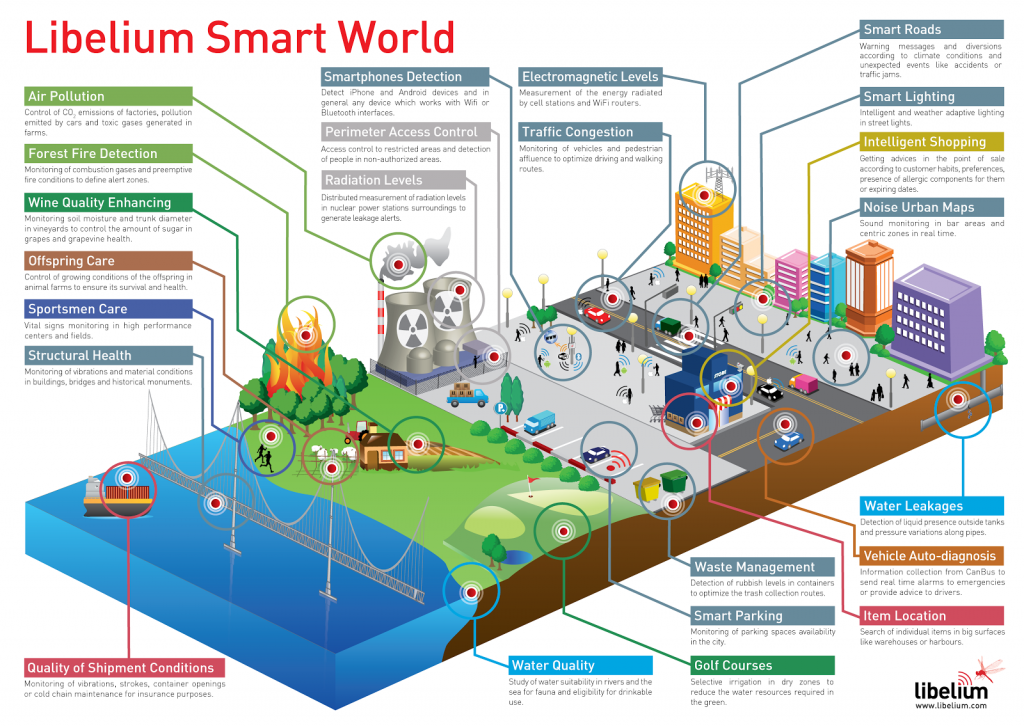
\includegraphics[scale=0.3]{libelium_smart_world}  
	\caption[Ilustrasi Pemanfaatan \textit{Wireless Sensor Network}]{Ilustrasi Pemanfaatan \textit{Wireless Sensor Network}} 
	\label{fig:smartworld} 
\end{figure} 

\subsection{Node Sensor}
%ganti gambar strutur sensor node
\subsubsection{Struktur Node Sensor}
Setiap node sensor memiliki kemampuan deteksi, komputasi dan komunikasi. Node sensor memiliki lima komponen utama yaitu \textit{controller}, \textit{memory}, \textit{sensor and actuator}, \textit{communication device}, dan \textit{power supply}, (Gambar~\ref{fig:structure_sensor_node}). Semua komponen akan bekerja secara seimbang dalam melakukan sensing, komputasi, komunikasi, dan menjaga penggunaan energi seminimal mungkin. 

\begin{figure} [H]
	\centering  
	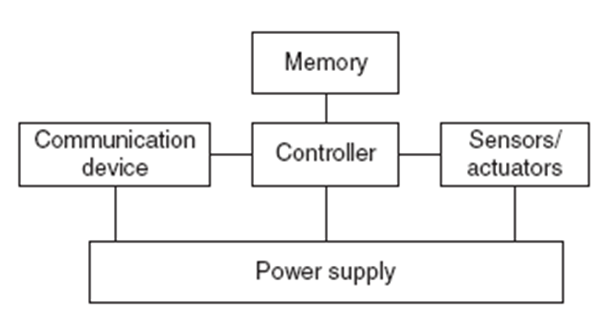
\includegraphics[scale=0.3]{structure_sensor_node}  
	\caption[Struktur Node Sensor]{Struktur Node Sensor} 
	\label{fig:structure_sensor_node} 
\end{figure} 

\subsubsection{Controller}
Controller adalah inti utama pada node sensor. Controller mengumpulkan data dari sensor dan memproses data tersebut hingga menentukan kapan dan kemana data tersebut dikirim. Controller menerima data dari node sensor lain. Pada controller biasanya terdapat microcontroller atau microprocessor yang mengatur dan melakukan komputasi data dari node sensor. Microcontroller ini juga dapat mengurangi penggunaan energi dengan masuk ke sleep states yang berarti hanya bagian dari controller saja yang aktif.

Beberapa microcontroller yang digunakan dalam Wireless Sensor Node:
\begin{itemize}
	\item Intel StrongARM (32-bit RISC, up to 206 MHz)
	\item Texas Instrument MSP 430 (16-bit RISC, up to 4 MHz,RAM 2-10 kB)
	\item Atmel Atmega 128L (8-bit)
\end{itemize}

\subsubsection{Memory}
Random Access Memory (RAM) digunakan untuk menyimpan sementara hasil yang didapat dari sensor. RAM juga menyimpan sementara paket dari node sensor lain. Jika power supply terjadi masalah maka data pada RAM ini akan hilang. Ini merupakan salah satu kekurangan dari penggunaan RAM. Maka untuk menyimpan kode program digunakanlah Read Only Memory (ROM). ROM ini biasa disebut Electrically Erasable Programmable Read-Only Memory (EEPROM) atau Flash Memory. Flash memory dapat menyimpan data jika suatu saat data pada RAM hilang atau energi sudah habis (intermediate storage).

\subsubsection{Communication Device}
\textit{Communication Device} digunakan untuk bertukar data antar node sensor. Pada aplikasi Wireless Sensor Network, Radio Frequency(RF)-based adalah media komunikasi yang paling relevan saat ini. RF-based mendukung jangkauan yang jauh, data rate yang tinggi, dapat menerima error rate pada penggunaan energi, dan tidak perlu saling mengetahui posisi antara penerima dan pengirim.

Pada node sensor dibutuhkan transmitter dan receiver untuk menerima dan mengirim data. Kedua hal ini dapat digabung dan disebut dengan transceiver. Tugas transceiver adalah mengubah stream bit dari microcontroller dan mengubahnya menjadi gelombang radio. Selain itu transceiver juga dapat mengubah gelombang radio menjadi stream bit.

\subsubsection{Sensor dan Actuator}
Sensor dan Actuator adalah hal yang penting pada Wireless Sensor Network. Tanpa sensor dan actuator maka node sensor tidak berguna dan tidak dapat digunakan. Tabel~\ref{tab:sensor} adalah jenis - jenis sensor yang dapat dimiliki node sensor. Sensor dikategorikan menjadi tiga:
\begin{enumerate}
	\item \textbf{Passive, omnidirectional sensors} Sensor ini dapat mengukur kualitas dari lingkungan fisik tempat node sensor tersebut tanpa mengubah lingkungannya. Beberapa sensor dikategori ini \textit{self-powered}, sensor mendapatkan energi yang mereka butuhkan dari lingkungannya. Energi ini digunakan untuk memperkuat sinyal analog. \textit{Omnidirectional} berarti tidak ada arah pada sensor ini. Sensor akan memancarkan sinyalnya ke segala arah. Contoh sensor ini adalah termometer, sensor cahaya, sensor getaran, mikrofon, sensor kelembapan, sensor tekanan udara, sensor deteksi asap, dan lain-lain.
	\item \textbf{Passive, narrow-beam sensors} Sensor ini memiliki sifat yang sama yaitu pasif, tidak mengubah lingkungannya. Sensor ini dapat melakukan gerakan dan memiliki arah atau daerah pengukuran. Contoh dari sensor ini adalah kamera yang bisa mengukur sesuai dengan arah yang dituju.
	\item \textbf{Active Sensor} Sensor ini aktif dalam memeriksa lingkungannya. Contoh dari sensor ini adalah sonar, radar atau sensor seismik. Sensor ini menghasilkan gelombang dengan ledakan kecil untuk melakukan deteksi.
\end{enumerate}

Actuator jumlahnya beragam seperti sensor. Actuator adalah penerima sinyal dan yang mengubahnya menjadi aksi fisik. Contoh aktuator adalah LED, yang mengubah listrik menjadi cahaya dan motor (electrical motor) juga mengubah listrik menjadi gerakan.

\begin{table} [H]
	\centering 
	\caption{Jenis - jenis sensor yang dapat dimiliki node sensor}
	\label{tab:sensor}
	\begin{tabular}{|c|c|c|}
		\toprule
		Sensor & Sense Event & Remark\\

		\midrule
		Accelerometer & & \\
		Acoustic emission sensor &  & \\
		Acoustic sensor &  & \\
		Capacitance sensor &  & \\
		ECG &  & \\
		EEG &  & \\
		EMG &  & \\
		Electrical/electromagnetic sensor &  & \\
		Gyroscope &  & \\
		Humidity Sensor &  & \\
		Infrasonic sensor &  & \\
		Magnetic sensor &  & \\
		Oximeter &  & \\
		pH sensor &  & \\
		Photo acoustic spectroscopy &  & \\
		Piezoelectric cylinder  &  & \\
		Soil moisture sensor &  & \\
		Temperature sensor &  & \\
		Barometer sensor &  & \\
		Passive infrared sensor &  & \\
		Seismic sensor &  & \\
		Oxygen sensor &  & \\
		Blood flow sensor &  & \\

		\bottomrule
		
	\end{tabular} 
\end{table}

\subsubsection{Power Supply}
Power supply atau sumber energi pada Wireless Sensor Network bisa berasal dari dua cara yaitu \textbf{\textit{storing energy}} dan \textbf{\textit{energy scavenging}}. \textit{Storing energy} adalah dengan menggunakan baterai sebagai sumber energinya. Baterai yang digunakan dapat diisi ulang maupun yang tidak dapat diisi ulang. \textit{Energy scavenging} digunakan saat membuat Wireless Sensor Network yang akan digunakan dalam waktu yang lama. Dibutuhkan energi yang bisa dikatakan tidak terbatas. Salah satu cara \textit{energy scavenging} adalah \textit{Photovoltaics}. \textit{photovoltaics} dapat disebut juga \textit{solar cell} yang memanfaatkan cahaya matahari dan mengubahnya menjadi energi sebagai pembangkit daya. Cara lain yang bisa digunakan adalah pemanfaatan angin dan air untuk mengerakan kincir atau turbin yang akan menghasilkan listrik dan digunakan sebagai sumber energi pada node sensor.

\subsection{Arsitektur dan Topologi Wireless Sensor Network}
Pada \textit{Wireless Sensor Network} biasanya akan terdapat banyak node sensor yang disebar pada suatu tempat. Terdapat satu atau lebih \textit{sink node} atau \textit{base station} dalam area sensing tersebut (Gambar~\ref{fig:arsitektur}). \textit{sink node} atau \textit{base station} adalah node sensor yang bertugas untuk mendapatkan data dari node sensor lain. Dalam membuat \textit{Wireless Sensor Network} perlu diperhatikan arsitektur dan topologi yang akan digunakan. Tidak semua topologi jaringan komputer dapat digunakan untuk \textit{Wireless Sensor Network}. 

Ada banyak topologi pada jaringan sensor (\textit{sensor network}). Pada jaringan sensor dengan menggunakan kabel topologi yang sering digunakan adalah topologi \textit{star}, \textit{line}, atau \textit{bus}. Sedangkan pada jaringan sensor tanpa kabel (WSN) topologi yang biasa digunakan adalah \textit{star}, \textit{tree}, atau \textit{mesh}. 

\subsubsection{Topologi Point-to-Point}
Topologi point-to-point adalah topologi yang menghubungkan dua titik (Gambar~\ref{fig:point2point}). Topologi point-to-point dibagi menjadi dua yaitu permanent point-to-point dan switched point-to-point. Permanent point-to-point adalah koneksi perangkat keras antara dua titik dan tidak dapat diubah. Switched point-to-point adalah koneksi point-to-point yang dapat berpindah antara node yang berbeda. 
\begin{figure} [H]
	\centering  
	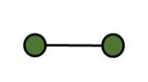
\includegraphics[scale=1.3]{point2point}  
	\caption[Topologi Point-to-Point]{Topologi Point-to-Point} 
	\label{fig:point2point} 
\end{figure} 

\subsubsection{Topologi Bus}
Topologi bus seperti pada Gambar~\ref{fig:bus} akan terdiri dari node-node dan sebuah jalur. Setiap node akan terhubung dengan jalur yang sama. Untuk mengirim data atau komunikasi akan dilakukan bergantian antar node. Kekurangan dari topologi bus ini adalah jika suatu saat jalur / bus ini mengalami kerusakan maka setiap node tidak dapat berkomunikasi lagi.
\begin{figure} [H]
	\centering  
	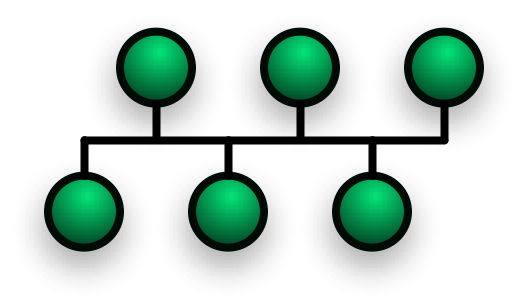
\includegraphics[scale=0.2]{bus}  
	\caption[Topologi Bus]{Topologi Bus} 
	\label{fig:bus} 
\end{figure} 

\subsubsection{Topologi Ring}
Pada topologi ring node akan disusun dengan bentuk melingkar (Gambar~\ref{fig:ring}). Setiap node akan terkoneksi dengan dua node lain. Transfer data terjadi dengan cara data akan berjalan dari satu node ke node lain mengikuti jalur melingkar tersebut hingga menemukan node tujuan yang tepat. Topologi ini mudah untuk diimplementasikan tapi kekurangan dari topologi ring adalah saat ada node yang rusak maka perlu biaya lebih untuk memperbaikinya. Biasanya node untuk menangani kegagalan komunikasi akibat node yang rusak, akan di atur komunikasi node tidak hanya satu arah tetapi dapat ke arah sebaliknya.
\begin{figure} [H]
	\centering  
	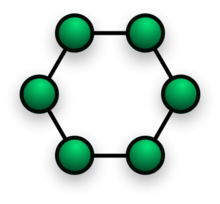
\includegraphics[scale=0.4]{ring}  
	\caption[Topologi Ring]{Topologi Ring} 
	\label{fig:ring} 
\end{figure} 

\subsubsection{Topologi Star}
Topologi star terdiri dari satu node yang berada di tengah biasanya berupa hub atau switch seperti pada Gambar~\ref{fig:star}. Setiap node akan terkoneksi dengan node yang berada di tengah ini. Saat node akan berkomunikasi dengan node lain, node tersebut harus mengirimkan data tersebut ke node yang ada ditengah dahulu dan node yang ditengah ini akan meneruskan data tersebut ke node tujuan. Yang paling penting pada topologi ini adalah node yang berada di tengah, karena semua komunikasi harus melalui node tersebut. Jika node tengah mengalami kerusakan maka tidak akan terjadi komunikasi antar node pada jaringan tersebut.
\begin{figure} [H]
	\centering  
	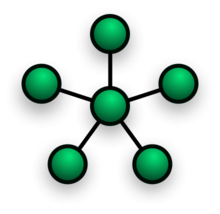
\includegraphics[scale=0.4]{star}  
	\caption[Topologi Star]{Topologi Star} 
	\label{fig:star} 
\end{figure} 

\subsubsection{Topologi Tree}
Pada topologi tree node-node akan disusun secara hierarki dengan satu node yang berada pada level paling atas sebagai \textit{root node} (Gambar~\ref{fig:tree}). \textit{Root node} akan terhubung dengan satu atau lebih node level dibawahnya. Dengan topologi tree lebih mudah untuk melakukan identifikasi dan meminimalisir kesalahan, namun jika tree sudah sangat besar / level tree sudah sangat banyak maka akan sulit untuk mengaturnya.
\begin{figure} [H]
	\centering  
	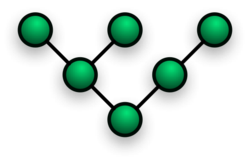
\includegraphics[scale=0.5]{tree}  
	\caption[Topologi Tree]{Topologi Tree} 
	\label{fig:tree} 
\end{figure} 

\subsubsection{Topologi Mesh}
Topologi mesh dibagi menjadi dua yaitu partially connected mesh dan fully connected mesh. Pada partially connected mesh (Gambar~\ref{fig:mesh_partial}), node akan terhubung dengan lebih dari satu node. Pada fully connected mesh (Gambar~\ref{fig:mesh_fully}), setiap node akan terhubung dengan semua node lain pada jaringan tersebut
\begin{figure} [H]
	\centering  
	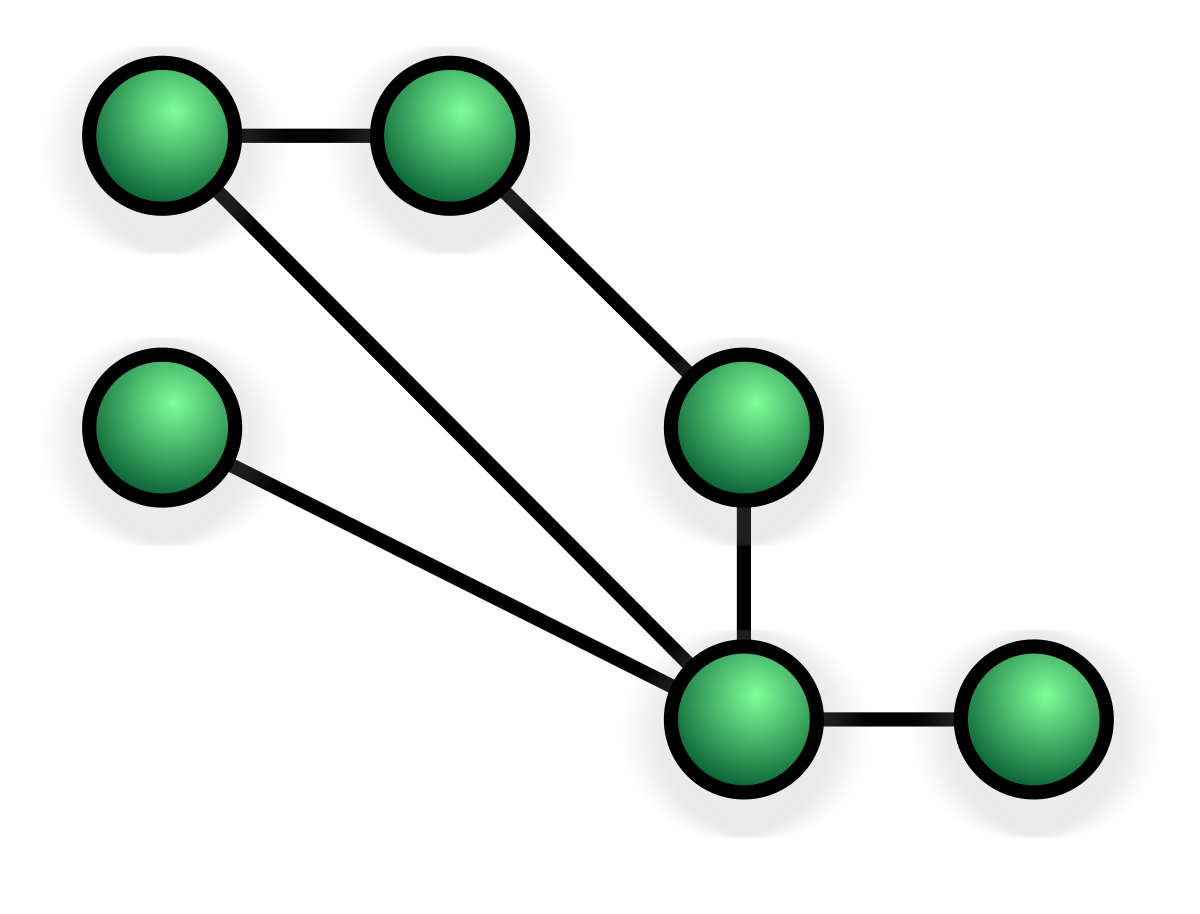
\includegraphics[scale=0.1]{mesh_partial}  
	\caption[Topologi Partially Connected Mesh]{Topologi Partially Connected Mesh} 
	\label{fig:mesh_partial} 
\end{figure} 
\begin{figure} [H]
	\centering  
	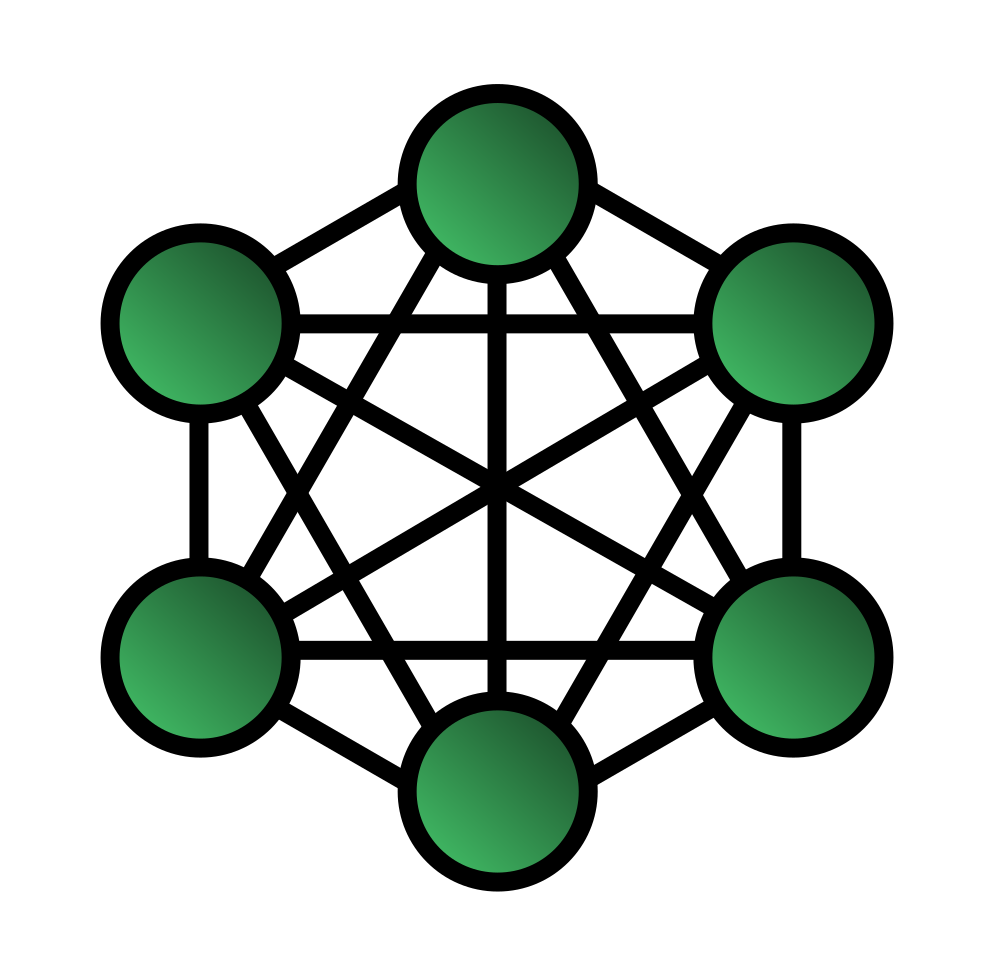
\includegraphics[scale=0.1]{mesh_fully}  
	\caption[Topologi Fully Connected Mesh]{Topologi Fully Connected Mesh} 
	\label{fig:mesh_fully} 
\end{figure} 

Arsitektur yang biasanya dipakai pada \textit{Wireless Sensor Network} adalah \textbf{arsitektur flat / peer-to-peer} dan \textbf{arsitektur hierarki}. Selain itu dalam membangun \textit{Wireless Sensor Network} perlu juga diperhatikan jalur komunikasi yang digunakan untuk menghubungkan antar node sensor saat transfer data. Untuk area \textit{sensing} yang tidak terlalu luas dan hanya menggunakan sedikit node sensor dapat menggunakan cara komunikasi \textbf{\textit{single hop}}. Sedangkan untuk daerah yang luas dan memerlukan banyak node sensor dapat menggunakan cara komunikasi \textbf{\textit{multi hop}}. 

\begin{figure} [H]
	\centering  
	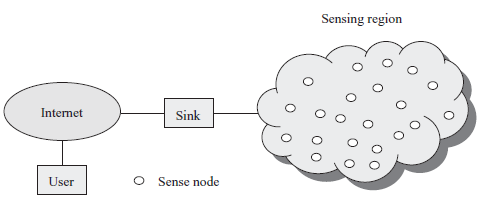
\includegraphics[scale=1]{arsitektur}  
	\caption[Arsitektur Wireless Sensor Network]{Arsitektur Wireless Sensor Network} 
	\label{fig:arsitektur} 
\end{figure} 

\subsubsection{Single-Hop dan Multi-Hop}
Untuk mengirim data ke sink node setiap node sensor dapat menggunakan single-hop long-distance transmission. Single-hop long-distance ini berarti setiap node sensor akan mengirimkan data ke sink node hanya satu kali lompatan walaupun jarak antara sink node dengan node sensor itu sangat jauh. Dalam jaringan sensor, penggunaan energi paling besar adalah saat melakukan komunikasi dibandingan saat sensing. Penggunaan energi akan semakin bertambah jika jarak sink dan node sensor semakin jauh. Untuk menangani masalah tersebut muncul protokol multi-hop.

Pada protokol multi-hop node sensor akan disusun saling berdekatan dan terhubung dengan yang lain. Jadi saat akan berkomunikasi dengan sink node, node sensor harus mengirimkan data tersebut ke node sensor tetangganya dan diteruskan hingga sampai ke sink node. Karena jarak yang saling berdekatan maka penggunaan energi dapat efektif. Single-hop dan multi-hop ini dapat digunakan dengan topologi flat maupun hierarki sesuai dengan kebutuhan sistem.

\subsubsection{Arsitektur Flat / Peer-to-Peer}
Pada arsitektur flat, setiap node sensor memiliki peran atau \textit{role} yang sama dalam melakukan \textit{sensing}. Secara fungsional hanya terdapat dua macam node sensor pada arsitektur flat, yaitu \textit{source node} dan \textit{sink node}. Karena jumlah node sensor yang banyak maka tidak mungkin menentukan \textit{global identified} untuk setiap node sensor pada jaringan ini. Untuk mendapatkan data dilakukan dengan cara \textit{sink node} melakukan pengiriman data ke semua node sensor pada area \textit{sensing} dengan cara \textit{flooding} dan hanya node sensor yang sesuai yang akan merespon \textit{sink node}. Setiap node sensor mengirimkan data ke \textit{sink node} dengan \textit{multi hop} dan melalui node tetangganya yang terhubung dengannya untuk meneruskan data (Gambar~\ref{fig:flat}).
% gambar flat
\begin{figure} [H]
	\centering  
	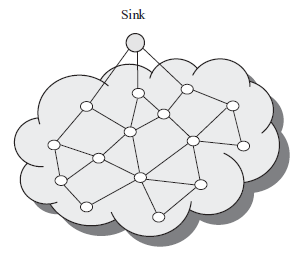
\includegraphics[scale=0.7]{flat}  
	\caption[Arsitektur flat pada \textit{Wireless Sensor Network}]{Arsitektur flat pada \textit{Wireless Sensor Network}} 
	\label{fig:flat} 
\end{figure} 

\subsubsection{Arsitektur Hierarki}
Pada arsitektur hierarki, semua node sensor dikelompokan ke dalam cluster-cluster. Terdapat cluster head pada setiap cluster. Cluster head ini yang mengumpulkan data dari setiap node sensor di bawahnya dan meneruskan data yang telah diterima ke base station atau sink. Hal yang perlu diperhatikan pada arsitektur hierarki adalah pemilihan node sensor sebagai cluster head dan node sensor yang melakukan sensing. Penggunaan energi yang paling besar dalam Wireless Sensor Network ini adalah saat melakukan komunikasi yaitu saat mengirimkan data ke node sensor lain. Maka untuk node sensor yang memiliki energi kecil dapat digunakan untuk sensing, karena node sensor sensing ini hanya melakukan komunikasi ke cluster head. Cluster head harus memiliki energi atau daya yang lebih banyak, karena cluster head akan bertugas menerima hasil sensing node sensor di bawahnya dan meneruskan data ke sink node. 

Masalah yang utama pada clustering ini adalah pemilihan cluster head dan bagaimana cara mengatur setiap cluster. Terdapat beberapa cara untuk membuat clustering ini. Bedasarkan jarak antara cluster head dengan cluster member, dapat dibuat clustering dengan single hop atau multi hop seperti pada Gambar~\ref{fig:cluster_single} dan Gambar~\ref{fig:cluster_multi}. Sedangkan jika berdasarkan jumlah tier dapat dibangun clustering single tier atau multi tier (Gambar~\ref{fig:cluster_multitier}).
\begin{figure} [H]
	\centering  
	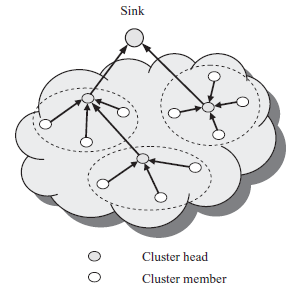
\includegraphics[scale=0.8]{cluster_single}  
	\caption[Arsitektur hierarki pada \textit{Wireless Sensor Network} dengan \textit{single hop} terhadap \textit{Cluster Head}]{Arsitektur hierarki pada \textit{Wireless Sensor Network} dengan \textit{single hop} terhadap \textit{Cluster Head}} 
	\label{fig:cluster_single} 
\end{figure} 
\begin{figure} [H]
	\centering  
	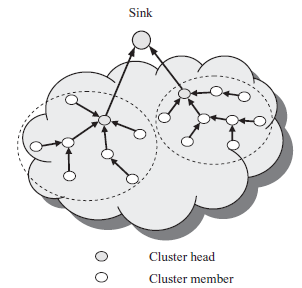
\includegraphics[scale=0.8]{cluster_multi}  
	\caption[Arsitektur hierarki pada \textit{Wireless Sensor Network} dengan \textit{multi hop}]{Arsitektur hierarki pada \textit{Wireless Sensor Network} dengan \textit{multi hop}} 
	\label{fig:cluster_multi} 
\end{figure} 
\begin{figure} [H]
	\centering  
	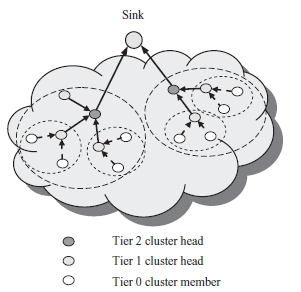
\includegraphics[scale=0.8]{cluster_multitier}  
	\caption[Clsutering dengan multi tier]{Clsutering dengan multi tier} 
	\label{fig:cluster_multitier} 
\end{figure}

%00 wireless sensor network hal 293
\subsection{Sistem Operasi}
Setiap node sensor memerlukan sistem operasi (OS) untuk mengontrol perangkat keras dan perangkat lunak. Sistem operasi tradisional tidak dapat digunakan pada WSN. Pada sistem operasi tradisional digunakan untuk mengatur proses, memory, CPU time, dan file system. Terdapat beberapa hal yang harus ditangani oleh sistem operasi dalam WSN yaitu:
\begin{enumerate}
	\item WSN memerlukan real-time scheduler. Data yang didapat harus segera dikirim atau diproses.
	\item Pengaturan memori karena memory pada WSN sangat kecil.
	\item Pengaturan data yang efisien terkait dengan microprocessor dan memori yang terbatas
	\item Mendukung kode pemrograman yang efisien dan reliable karena dapat terjadi perubahan kode saat implementasi.
	\item Mendukung pengaturan sumber daya untuk menambah waktu hidup dari node sensor dan meningkatkan performa dengan sleep time atau wake up time saat terdapat interupsi dari lingkungan.
	\item Mendukung antarmuka untuk pemrograman dan antarmuka perangkat lunak. 
\end{enumerate}

Beberapa sistem operasi yang umum digunakan pada WSN antara lain :
\begin{enumerate}
	\item TinyOS
	\item Contiki
	\item LiteOS
\end{enumerate}

%Operating SYstem for WSN a survey - hal 7
\subsubsection{TinyOS}
TinyOS adalah sistem operasi open-source yang digunakan pada WSN. TinyOS dapat menjalankan program dengan memori yang sangat kecil. Ukurannya hanya 400 Byte. Komponen librari TinyOS terdiri dari protokol jaringan, layanan distribusi sensor, driver sensor, dan software pengamatan data sensor yang dapat digunakan untuk melakukan monitoring jaringan sensor. Gambar~\ref{fig:tinyOS} adalah arsitektur pada TinyOS. 
\begin{figure} [H]
	\centering  
	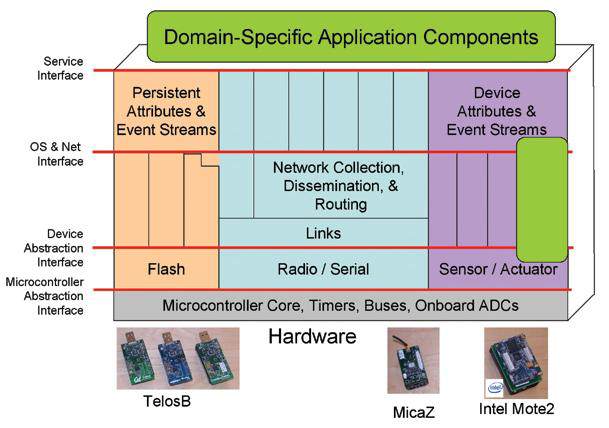
\includegraphics[scale=0.5]{tinyOS}  
	\caption[Arsitektur TinyOS]{Arsitektur TinyOS} 
	\label{fig:tinyOS} 
\end{figure}

%Operating SYstem for WSN a survey - hal 11
\subsubsection{Contiki}
Contiki adalah sistem operasi open-source dengan Bahasa Pemrograman C yang digunakan pada WSN. Contiki sudah mendukung multitasking pada suatu proses. Pengaturan Contiki hanya memerlukan 2KB dari RAM dan 40KB dari ROM. Fitur yang dimiliki oleh Contiki antara lain: multitasking, multithreading, jaringan TCP/IP, IPv6, GUI, Web Browser, Web Server, telnet, dan komputasi jaringan virtual. Gambar~\ref{fig:contiki} adalah arsitektur pada Contiki
\begin{figure} [H]
	\centering  
	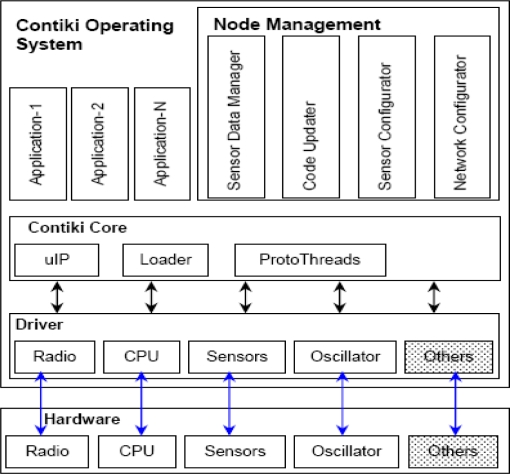
\includegraphics[scale=3]{contiki}  
	\caption[Arsitektur Contiki]{Arsitektur Contiki} 
	\label{fig:contiki} 
\end{figure}

%Operating SYstem for WSN a survey - hal 23
\subsubsection{LiteOS}
LiteOS adalah sistem operasi mirip UNIX yang didisain untuk WSN. Tujuan dibuat LiteOS adalah membuat sistem operasi yang mirip dengan UNIX agar lebih lebih familiar dengan paradigma pemrograman UNIX. Pada LiteOS terdapat sistem berkas yang hiearki, dan mendukung Bahasa Pemrograman LiteC++ dan UNIX Shell. LiteOS dapat digunakan untuk MicaZ yang memiliki 8 Mhz CPU, 128 byte flash, dan 4KB RAM. LiteOS memiliki tiga komponen utama yaitu: LiteShell, LiteFS, dan Kernel. Gambar~\ref{fig:contiki} adalah arsitektur pada LiteOS
\begin{figure} [H]
	\centering  
	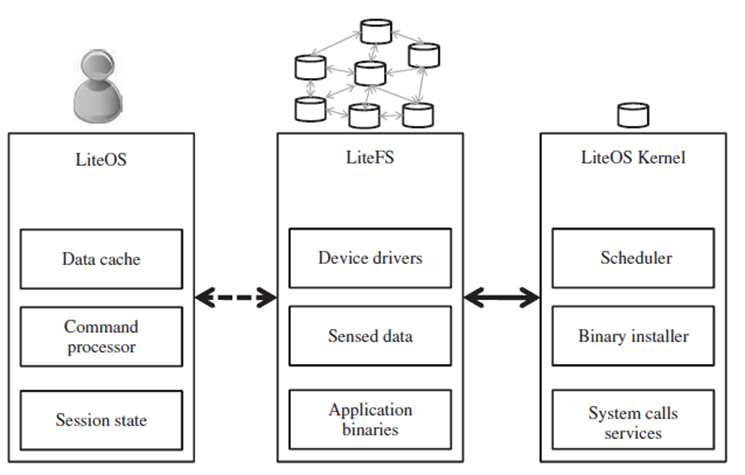
\includegraphics[scale=0.4]{liteOS}  
	\caption[Arsitektur LiteOS]{Arsitektur LiteOS} 
	\label{fig:liteOS} 
\end{figure}

Perbandingan dari TinyOS, Contiki, dan LiteOS dapat dilihat pada Tabel~\ref{tab:perbandinganOS} berikut ini:
\begin{table}[H] %atau h saja untuk "kira kira di sini"
	\centering 
	\caption{Tabel Perbandingan Sistem Operasi}
	\label{tab:perbandinganOS}
	\begin{tabular}{c|c|c|c|c}
		\toprule
		Operating System & Programming Paradigm & Scheduling & Memory Allocation & System Call\\

		\midrule
		TinyOS & Event-based & FIFO & Static & Not Available\\
		Contiki & Predominant event-based & FIFO & Dynamic & Runtime libraries\\
		LiteOS & Thread-based & Priority-based scheduling with optional round-robin support & Dynamic & A host of system calls available to the user (file, process, environment, debugging, and device command) 	\\

		\bottomrule
		
	\end{tabular} 
\end{table}

%\section{Preon 32 Virtenio}

%data transfer 

\subsection{Protokol Stack pada Wireless Sensor Network}
Wireless Sensor Network memiliki lima layer protokol: physical layer, data link layer, network layer, transport layer, dan application layer, seperti pada Gambar~\ref{fig:layer}. 
\begin{figure} [H]
	\centering  
	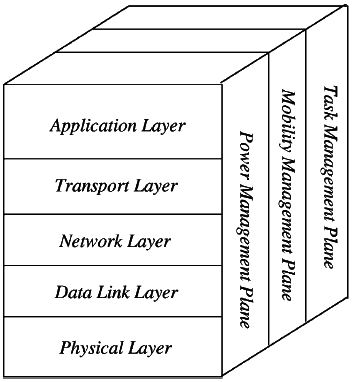
\includegraphics[scale=0.5]{layer}  
	\caption[Layer pada \textit{Wireless Sensor Network}]{Layer pada \textit{Wireless Sensor Network}} 
	\label{fig:layer} 
\end{figure} 

\subsubsection{Physical Layer}
Physical layer bertanggung jawab untuk mengubah bit stream dari data link layer menjadi sinyal agar bisa dilakukan transmisi melalui media komunikasi yang ada (transceiver). Pemilihan media dan frekuensi adalah hal yang penting dalam komunikasi antar node sensor. Salah satu cara yang bisa digunakan adalah dengan menggunakan radio frekuensi (RF). Jaringan sensor memerlukan biaya yang kecil, ukuran yang kecil, dan penggunaan daya yang kecil untuk tranceivernya. Karena itu banyak yang menggunakan Radio Frequency (RF) untuk desain perangkat keras node sensornya.

\subsubsection{Data Link Layer}
Data link layer bertanggung jawab untuk aliran data multiplexing, membentuk data frame, mendeteksi data frame, medium access, dan mengatur kesalahan saat transmisi data. Fungsi paling penting data link layer adalah Medium Access Control (MAC). Protokol MAC menentukan kapan node sensor mengakses media untuk mengirim data, melakukan kontrol dan mengatur paket ke node sensor lain. Hal itu dilakukan agar tidak terjadi paket yang bertabrakan. 

\subsubsection{Network Layer}
Network layer bertanggung jawab untuk routing dari node sensor ke sink node. Pada WSN node sensor tersebar pada suatu tempat untuk melakukan sensing. Data sensing tersebut harus dikirimkan ke sink node untuk diolah. Dalam mengirimkan data tersebut dapat menggunakan single hop atau multi hop. Dalam mengirim data diperlukan protokol routing yang hemat energi.

\subsubsection{Transport Layer}
Secara umum transport layer bertanggung jawab untuk pengiriman data yang reliable antara node sensor dan sink node. Protokol transport yang biasa tidak bisa diterapkan pada WSN tanpa modifikasi. Setiap jaringan sensor memiliki fungsi khusus. Untuk aplikasi yang berbeda memerlukan kebutuhkan reliabilitas yang berbeda. Pengiriman data pada WSN dibagi menjadi dua yaitu: downstream dan upstream. Upstream berarti node sensor mengirimkan hasil sensing ke sink node. Downstream berarti data berasal dari sink node contohnya, queries, dan perintah-perintah yang dikirimkan ke setiap node sensor. Aliran data yang reliable untuk kedua jenis pengiriman ini mungkin berbeda. Pada upstream reliable data dapat ditoleransi karena sensor akan melakukan sensing terus menerus dan dapat terjadi pengulangan data sehingga data yang hilang tadi dapat dikoreksi. Sedangkan pada downstream memerlukan 100\% pengiriman data yang reliable. 

\subsubsection{Application Layer}
Application layer meliputi berbagai macam protokol yang ada pada layer ini untuk menjalankan berbagai macam aplikasi seperti query dissemination, node localization, time synchronization, dan network security. Protokol yang ada pada layer ini antara lain:
\begin{enumerate}
	\item Sensor management protocol (SMP) adalah protokol untuk melakukan pertukaran lokasi data, sinkornisasi node sensor, memindahkan node sensor, mengatur ulang node sensor, dan menyimpan status dari node sensor.
	\item Sensor query and data dissemination protocol (SQDDP) adalah protokol yang mendukung antarmuka aplikasi untuk memasukan query, merespon query, dan mengumpulkan respon.
	\item Sensor query and tasking language (SQTL) adalah protokol yang mendukung bahasa pemrograman pada WSN.
\end{enumerate}

\section{Protokol Transport}


\section{Prinsip Reliable Data Transfer pada Wireless Sensor Network}
\label{sec:reliable}
Banyak aplikasi jaringan komputer tidak hanya Wireless Sensor Network yang memerlukan pengumpulan data tanpa ada data yang hilang (loss). Terdapat empat cara yang dapat digunakan untuk membuat aplikasi transfer data yang reliable pada jaringan komputer:
\begin{enumerate}
	\item Link-Level Retransmission
	\item End-to-End Retransmission
	\item Erasure Code
	\item Alternative Route
\end{enumerate}

\subsection{Link-Level Retransmission}
Tingkat data yang hilang (loss) pada jaringan wireless lebih tinggi dibandingkan dengan jaringan kabel (wired). Jika persentase data hilang 10\% per hop, maka setelah 15 hop persentase menjadi 80\%. Saat pada hop ke-n terjadi loss data, maka semua pengiriman data sampai hop ke n-1 akan menjadi tidak berguna. Untuk mengirimkan paket hop ke-n lagi diperlukan sebanyak n-1 kali tambahan pengiriman jika berhasil. Jika menggunakan Link-Level Retransmission hanya dibutuhkan satu kali retransmission (pengiriman ulang) untuk sampai ke posisi yang sama. Untuk masalah efisien link-level retransmission adalah pilihan yang tepat.

Waktu pengiriman bergantung pada berapa jumlah retransmission dan Round trip time (RTT) yang bervariasi. Ini membuat End-to-End Retransmission tidak efisien karena tidak diketahui jumlah RTT. Untuk masalah paket yang loss, pengirim paket harus menyimpan buffer untuk waktu yang lama dan menunggu hingga menerima acknowledgement dari hop berikutnya. Menyimpan buffer pada memori bukan hal yang tepat pada WSN.

\subsection{End-to-End Retransmission}
End-to-End Retransmission adalah salah satu metode yang digunakan di Internet. Cara ini dapat memastikan reliable data tanpa harus mengetahui apa yang terjadi di tengah jaringan. Pada End-to-End Retransmission diperlukan handshake seperti pada komunikasi jaringan komputer. Pada awalnya data dikirim sebagai permintaan transfer. Jika penerima (receiver) memiliki cukup RAM, dan layer aplikasi dapat menerima data tersebut, maka receiver mengirimkan acknowledge untuk permintaan data tersebut. Saat koneksi sudah terbentuk, data yang sebenarnya dapat dikirim. Data tersusun dari beberapa round. Setiap round, pengirim (sender) mengirim paket yang hilang pada round sebelumnya. Diakhir setiap  round receiver mengirimkan acknowledge kepada sender yang berisi informasi paket yang hilang. Sender menerima acknowledge tersebut dan mengirim paket yang hilang tersebut. Untuk round pertama terdapat pengecualian karena semua pake pada round sebelumnya tidak ada (belum dikirim). 

\subsection{Erasure Code}

\subsection{Alternate Route}
Menambahkan rute alternatif untuk menangani kegagalan pada link atau jalur komunikasi adalah cara lain untuk meningkatkan keandalan. Saat link antara dua node sensor terjadi kerusakan maka data yang sedang dikirim akan dibuang (drop) sampai terdapat rute baru untuk mengirim data.

\section{Pengembangan Pemrograman pada Wireless Sensor Network}
\label{sec:pemrograman_wsn}


\newpage
\subsection{Tabel}  
Berikut adalah contoh pembuatan tabel. 
Penempatan tabel dan gambar secara umum diatur secara otomatis oleh \LaTeX{}, perhatikan contoh di file bab2.tex untuk melihat bagaimana cara memaksa tabel ditempatkan sesuai keinginan kita.

Perhatikan bawa berbeda dengan penempatan judul gambar gambar, keterangan tabel harus diletakkan di atas tabel!!
Lihat Tabel~\ref{tab:contoh1} berikut ini:

\begin{table}[H] %atau h saja untuk "kira kira di sini"
	\centering 
	\caption{Tabel contoh}
	\label{tab:contoh1}
	\begin{tabular}{cccc}
		\toprule
		& $v_{start}$ & $\mathcal{S}_{1}$ & $v_{end}$\\

		\midrule
		$\tau_{1}$ & 1 & 12& 20\\
		$\tau_{2}$ & 1 &  & 20\\
		$\tau_{3}$ & 1 & 9 & 20\\
		$\tau_{4}$ & 1 &  & 20\\

		\bottomrule
		
	\end{tabular} 
\end{table}
Tabel~\ref{tab:cthwarna1} dan Tabel~\ref{tab:cthwarna2} berikut ini adalah tabel dengan sel yang berwarna dan ada dua tabel yang bersebelahan. 
\begin{table}[H]
	\begin{minipage}[c]{0.49\linewidth}
		\centering
		\caption{Tabel bewarna(1)}
		\label{tab:cthwarna1}
		\begin{tabular}{ccccc}
			\toprule
			 & $v_{start}$ & $\mathcal{S}_{2}$ & $\mathcal{S}_{1}$ & $v_{end}$\\
			
			\midrule
			$\tau_{1}$ & 1 & 5 \cellcolor{green}& 12& 20\\
			$\tau_{2}$ & 1 & 8 \cellcolor{green}& & 20\\
			$\tau_{3}$ & 1 & 2/8/17 \cellcolor{green}& 9 & 20\\
			$\tau_{4}$ & 1 & \cellcolor{red}& & 20\\
			
			\bottomrule

		\end{tabular}
	\end{minipage}
	\begin{minipage}[c]{0.49\linewidth}
		
		\centering 
		\caption{Tabel bewarna(2)}
		\label{tab:cthwarna2}
		\begin{tabular}{ccccc}
			\toprule
			 & $v_{start}$ & $\mathcal{S}_{1}$ & $\mathcal{S}_{2}$ & $v_{end}$\\
			
			\midrule
			$\tau_{1}$ & 1 & 12& 5 \cellcolor{red} &20\\
			$\tau_{2}$ & 1 &  &  8 \cellcolor{green} &20\\
			$\tau_{3}$ & 1 & 9 & 2/8/17 \cellcolor{green} &20\\
			$\tau_{4}$ & 1 &   & \cellcolor{red} &20\\
			
			\bottomrule
		
		\end{tabular}
	\end{minipage}
\end{table}

 
\subsection{Kutipan}
\label{subs:kutipan} 
Berikut contoh kutipan dari berbagai sumber, untuk keterangan lebih lengkap, silahkan membaca file referensi.bib yang disediakan juga di template ini.
Contoh kutipan:
\begin{itemize}
	\item Buku:~\cite{berg:08:compgeom} 
	\item Bab dalam buku:~\cite{kreveld:04:GIS}
	\item Artikel dari Jurnal:~\cite{buchin:13:median}
	\item Artikel dari prosiding seminar/konferensi:~\cite{kreveld:11:median}
	\item Skripsi/Thesis/Disertasi:~\cite{lionov:02:animasi}~\cite{wiratma:10:following}~\cite{wiratma:22:later}
	\item Technical/Scientific Report:~\cite{kreveld:07:watertight}
	\item RFC (Request For Comments):~\cite{RFC1654}
	\item Technical Documentation/Technical Manual:~\cite{Z.500}~\cite{unicode:16:stdv9}~\cite{google:16:and7}
	\item Paten:~\cite{webb:12:comm}
	\item Tidak dipublikasikan:~\cite{wiratma:09:median}~\cite{lionov:11:cpoly}
	\item Laman web:~\cite{erickson:03:cgmodel}  
	\item Lain-lain:~\cite{agung:12:tango}
\end{itemize}    
  
\subsection{Gambar}

Pada hampir semua editor, penempatan gambar di dalam dokumen \LaTeX{} tidak dapat dilakukan melalui proses {\it drag and drop}.
Perhatikan contoh pada file bab2.tex untuk melihat bagaimana cara menempatkan gambar.
Beberapa hal yang harus diperhatikan pada saat menempatkan gambar:
\begin{itemize}
	\item Setiap gambar {\bf harus} diacu di dalam teks (gunakan {\it field} {\sc label})
	\item {\it Field} {\sc caption} digunakan untuk teks pengantar pada gambar. Terdapat dua bagian yaitu yang ada di antara tanda $[$ dan $]$ dan yang ada di antara tanda $\{$ dan $\}$. Yang pertama akan muncul di Daftar Gambar, sedangkan yang kedua akan muncul di teks pengantar gambar. Untuk skripsi ini, samakan isi keduanya.
	\item Jenis file yang dapat digunakan sebagai gambar cukup banyak, tetapi yang paling populer adalah tipe {\sc png} (lihat Gambar~\ref{fig:ularpng}), tipe {\sc jpg} (Gambar~\ref{fig:ularjpg}) dan tipe {\sc pdf} (Gambar~\ref{fig:ularpdf})
	\item Besarnya gambar dapat diatur dengan {\it field} {\sc scale}.
	\item Penempatan gambar diatur menggunakan {\it placement specifier} (di antara tanda  $[$ dan $]$ setelah deklarasi gambar.
	Yang umum digunakan adalah {\bf H} untuk menempatkan gambar {\bf sesuai} penempatannya di file .tex atau  {\bf h} yang berarti "kira-kira" di sini. \\
	Jika tidak menggunakan {\it placement specifier}, \LaTeX{} akan menempatkan gambar secara otomatis untuk menghindari bagian kosong pada dokumen anda.
	Walaupun cara ini sangat mudah, hindarkan terjadinya penempatan dua gambar secara berurutan. 	
	\begin{itemize}
		\item Gambar~\ref{fig:ularpng} ditempatkan di bagian atas halaman, walaupun penempatannya dilakukan setelah penulisan 3 paragraf setelah penjelasan ini.
		\item Gambar~\ref{fig:ularjpg} dengan skala 0.5 ditempatkan di antara dua buah paragraf. Perhatikan penulisannya di dalam file bab2.tex!
		\item Gambar~\ref{fig:ularpdf} ditempatkan menggunakan {\it specifier} {\bf h}.
	\end{itemize}
\end{itemize}
 
\dtext{17-18}
\begin{figure} 
	\centering  
	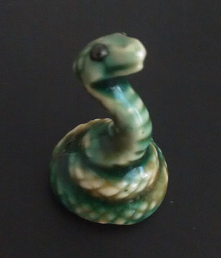
\includegraphics[scale=1]{ular-png}  
	\caption[Gambar {\it Serpentes} dalam format png]{Gambar {\it Serpentes} dalam format png} 
	\label{fig:ularpng} 
\end{figure} 

\dtext{19-20}
\begin{figure}[H]
	\centering  
	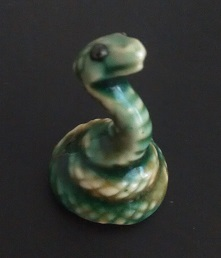
\includegraphics[scale=0.5]{ular-jpg}  
	\caption[Ular kecil]{Ular kecil} 
	\label{fig:ularjpg} 
\end{figure} 
\dtext{21-22}

\begin{figure}[ht] 
	\centering  
	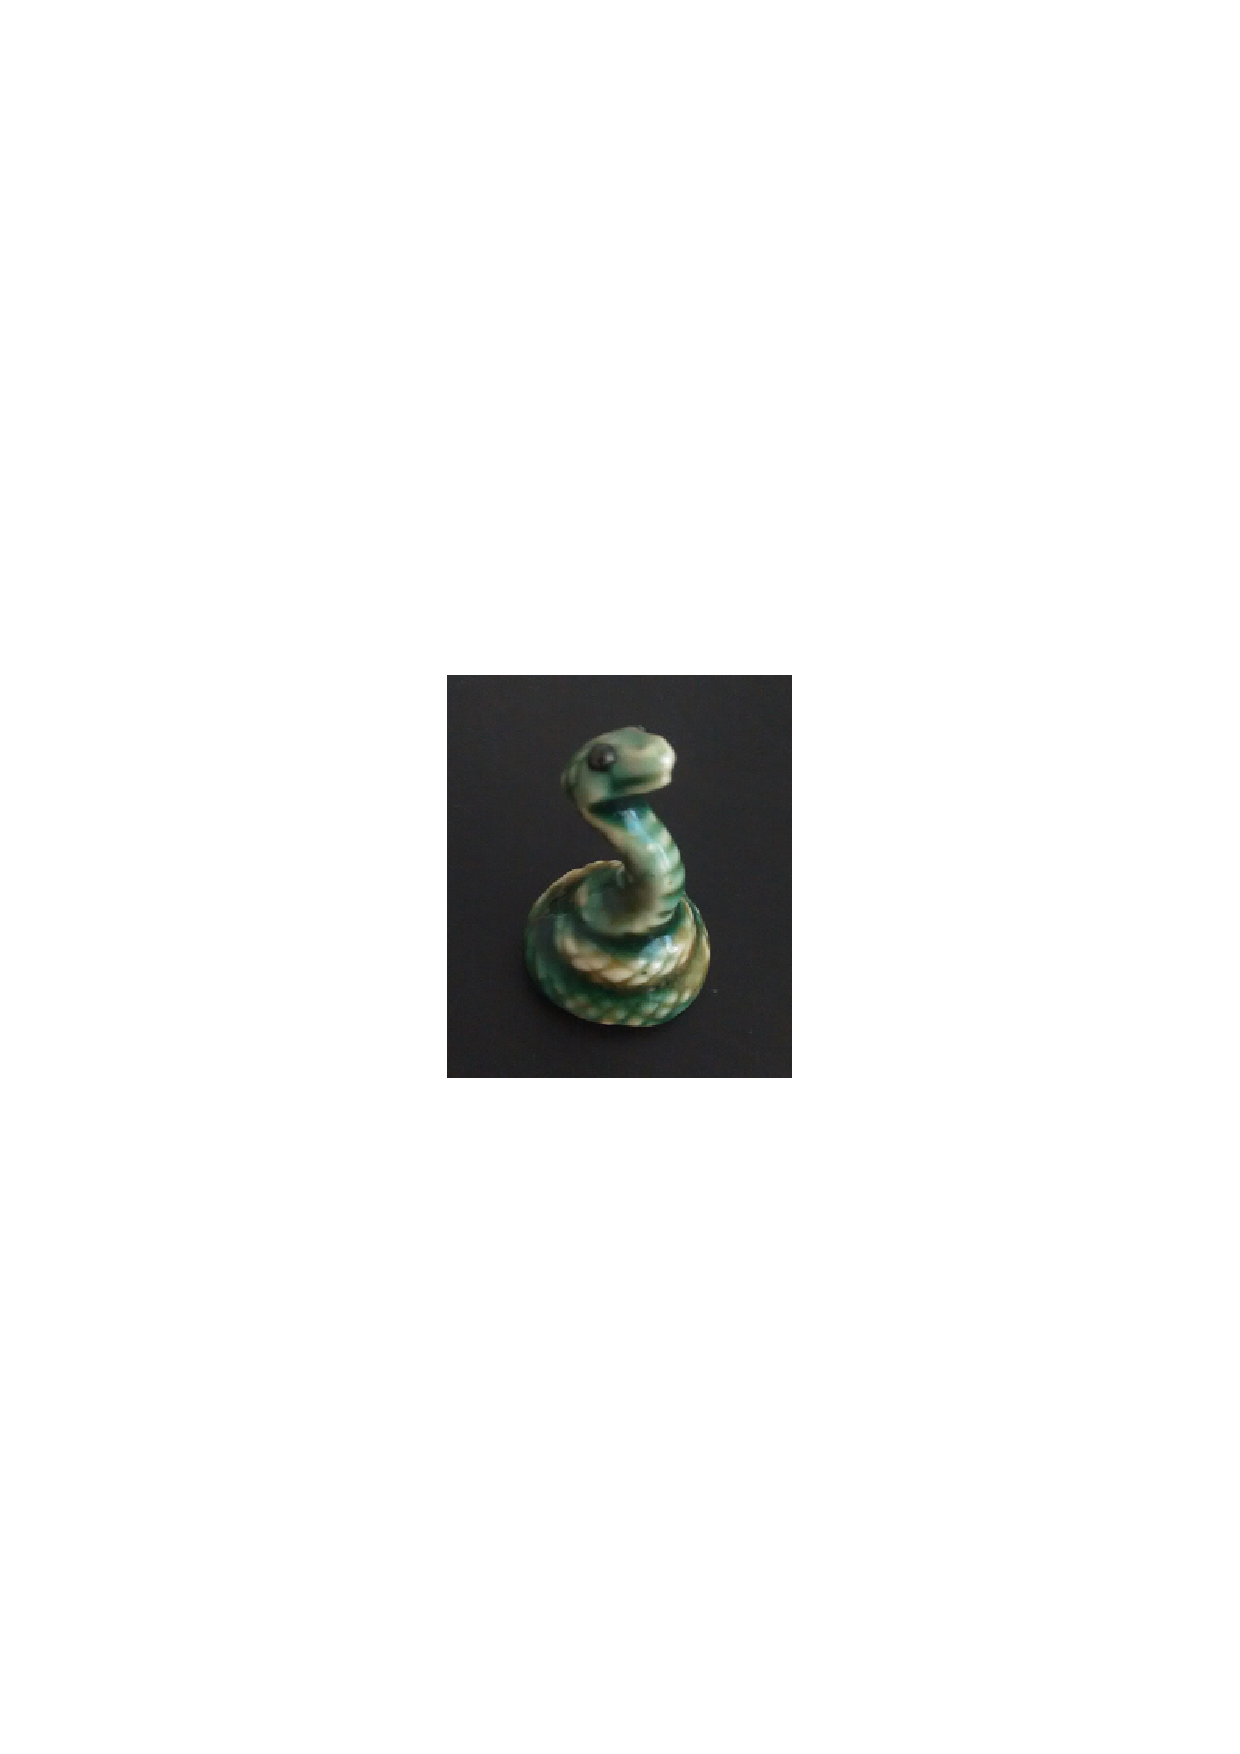
\includegraphics[scale=1]{ular-pdf}  
	\caption[ {\it Serpentes} betina]{ {\it Serpentes} jantan} 
	\label{fig:ularpdf} 
\end{figure} 
 
